\section{Question Answering over Knowledge Graphs}
\label{cap2:theoFrame/qakg}
Question Answering systems respond to the need to access information on the Web without 
detailed knowledge of Semantic Web technologies such as how data is structured (\RDF{}) or how to 
access data (\SPARQL{}). In particular, Question Answering systems (QASs) provide end-users with an 
intuitive and easy-to-use user interface, which hides the complexity behind the Semantic Web 
standards~\cite{qa:intro-UngerFC14}. These systems differ from traditional search engines such 
as Google in the final objective: search engines only return documents in which the answer can be 
potentially found, whereas a Question Answering system aims to return precise answers~\cite{qa:LopezUSM11}.

When we mention the task of Question Answering over Knowledge Graphs (QAKG), we refer to 
receiving a natural language question and returning an answer retrieved from one or more 
Knowledge Graphs (e.g. the first man to walk on the moon is Neil 
Amstrong\footnote{\url{https://www.wikidata.org/wiki/Q1615} in Wikidata.}). Though there is work 
that includes a wider context along with the question, such as hybrid questions or chain of 
questions, we focus only on the problem of responding to an individual question without further 
context besides the question itself.

Another consideration for defining the scope of Question Answering is the question and answer 
type a system aims to respond to/with. Among the types of questions for which a Question 
Answering system usually provides an answer are:

\begin{itemize}
    \item \textbf{Definition question}, refers to a definition of a subject or object (e.g. 
    \dquotesit{Who was Violeta Parra?}).
    \item \textbf{Factoid questions}, which are related to facts. This type of questions 
    includes three different variants:
    \begin{itemize}
        \item \textbf{Predicative questions} that refer to a specific object related to a predicate 
        such as who, what, where, how (e.g. \dquotesit{Who was the first man in space?}, 
        \dquotesit{What is the highest mountain in Chile?}).
        \item \textbf{List questions} that refer to all the answers that fulfill the fact being 
        asked (e.g. \dquotesit{Give me all the countries in America}).
        \item \textbf{Boolean questions} that refer to whether the fact being questioned is true 
        or not (e.g. \dquotesit{Was Gabriela Mistral a poet?}).
    \end{itemize}
\end{itemize}

In the context of Linked Data, a Question Answering system is limited to the information the 
available knowledge graphs can represent. For instance, questions not based on specific facts 
such as process questions (e.g. \dquotesit{How do I make a lemon pie?}) or opinion questions 
(e.g. \dquotesit{What do most Chileans think of global warming?}) cannot be answered.

Questions can also be classified depending on the answer type expected. One example is the work 
of Xin Li et al.~\cite{qa:LiR02}, which classify questions given five high-level categories: 
\textbf{entities} (e.g. event, color, animal, plant), \textbf{descriptions} (e.g. definition, 
manner, reason), \textbf{humans} (e.g. individual, group), locations (e.g. city, country, 
mountain) and numbers (e.g. count, date, distance, size). Another way is to classify questions 
according to its \textbf{focus} and \textbf{topic}, representing what the question is about. 
For instance, the question \dquotesit{What is the height of Aconcagua mountain?} focuses on the 
property height in the topic of geography while the question \dquotesit{What is the best 
height-increasing drug?} focuses on the same property, but a different topic, which is medicine.

According to Fu et al.~\cite{qa:FuQTLYS20abs-2007-13069}, current systems do not struggle with 
answering simple questions, i.e. questions that only require one subject-predicate-object 
triple fact, but complex questions are still a challenge for QAKG. A complex question usually 
is referred to as three types: questions under specific conditions (e.g. \dquotesit{Who was the 
president of Chile during the Great Recession of 2008?}), questions with more intentions (e.g. 
\dquotesit{Give the names of the Chilean national football team and the number of goals they have 
scored}), and questions requiring constraint inference (e.g. \dquotesit{What is the most 
expensive movie starring Pedro Pascal?}).

\subsection{QAKG approaches}
\label{cap2:theoFrame/qakg/approaches}
Though there is no standard approach for QAKG, most techniques or methods proposed follow a 
similar four-stage pipeline~\cite{qa:core-techniques-DiefenbachLSM18}. First, a question 
analysis stage includes techniques that extract information from the current question using 
purely syntactic features. Then, the phrase mapping stage defines techniques that identify KG 
resources for each named entity and its dependencies. Next, the disambiguation stage 
encapsulates techniques that rank and determine for each named entity the most relevant 
resources according to the context of the question. Lastly, the query construction stage 
considers techniques used to construct the \SPARQL{} query that should retrieve the final answer. 
In summary, most Question Answering systems are a combination of these four steps and vary with 
respect to which techniques are used to address each phase of the Question Answering process.

On the other hand, QAKG approaches can be classified according to which techniques their models 
are based on. The traditional QAKG models rely on predefined templates and manuals to parse 
questions~\cite{qa:core-techniques-DiefenbachLSM18}. However, these traditional approaches require 
a certain level of knowledge of linguistics, and tend to be difficult to scale. Therefore, recent 
work has focused more on two kinds of approaches: methods based on Information Retrieval methods 
and other ones based on Neural Semantic Parsing.

\subsubsection{Information Retrieval-based methods}
\label{cap2:theoFrame/qakg/approaches/infRetrieval}
Information Retrieval (IR) based models reduce the QA task to binary classification or sorting 
over candidate answers. An IR-based method usually begins by identifying relevant entities 
mentioned in the question. Then, it extracts topic-entity-centric subgraphs where all nodes are 
considered candidate answers. Next, candidates are scored using features that provide semantic 
relevance and help to select the final answers. Depending on how the feature representations 
are built, IR-based methods can be divided into those based on feature engineering and those 
based on representation learning.

Methods based on feature engineering rely on manually defined and extracted features. For 
example, Yao et al.~\cite{qa:YaoD14} extract four types of features based on the question’s 
syntactic information, which includes question words, question focus words, topic words, and 
central verbs. These features are used in a classification model to determine the final answer. 
However, building these features is time-consuming and is not able to capture the entire 
semantic information of questions.

Methods based on representation learning convert questions and candidate answers into vector 
representations and reduce QAKG to a semantic matching computation between representations of 
questions and their candidate answers. Some methods incorporate external knowledge to complement 
the representation information and address the incompleteness that the KG might 
have~\cite{qa:XuRFHZ16,qa:SunDZMSC18,qa:TrouillonWRGB16}. Some other methods incorporate a 
multi-hop reasoning process to handle more complex questions~\cite{qa:SukhbaatarSWF15,qa:MillerFDKBW16,qa:QiuWJZ20}.

Overall, IR-based models get rid of manually defined templates and rules, and can follow an 
end-to-end training. However, these methods lack model interpretability and are not able to 
handle complex questions that require constraint inference.

\subsubsection{Neural Semantic Parsing-based methods}
\label{cap2:theoFrame/qakg/approaches/neuSemParsing}
In this context, methods based on Semantic Parsing aims to convert natural languages into 
executable query languages. Methods based on Neural Semantic Parsing (NSP) rely on Neural 
Networks to enhance the parsing capacity and scalability, instead of relying on predefined 
templates or rules. Thus, these models aim to map unstructured questions to intermediate 
logical forms which are later converted to structured queries.

One approach is to use query graphs, which are graphs that encoded questions, have strong 
representation ability and share topological commonalities with knowledge graphs. One example 
is GraphParser, proposed by Reddy et al.~\cite{qa:ReddyLS14} which frames the Semantic Parsing 
problem as a Graph Matching problem. Derived from GraphParser, the Staged Query Graph 
Generation~\cite{qa:YihCHG15} (STAGG) and the Multiple Constraint Query Graph~\cite{qa:BaoDYZZ16} 
(MultiCG) were proposed. While STAGG proposed a different construction of the query graph based 
on a restricted subset of lambda-calculus in the graph representation, MultiCG extends STAGG to 
include more constraint types and operators in order to cover more complex questions. Since all 
these proposals rely on Entity Linking tools to initialize the query graph construction, 
Yu et al.~\cite{qa:YuYHSXZ17} assumes a poor performance of such tools and proposes a 
Hierarchical Residual BiLSTM with the goal of improving entity recognition accuracy.

On the other hand, other work proposes to use encoder-decoder models to reduce the Semantic 
Parsing task into a Sequence-to-Sequence problem. One example is the Seq-to-Tree model proposed 
by Dong et al.~\cite{nmt:DongL16} that uses a hierarchical tree-structured decoder to capture 
the structure of logical forms. Then, in order to take more advantage of the syntactic 
information of the input question, the Graph-to-Seq model was proposed by Xu et al.~\cite{qa:XuWWYCS18} 
to encode the question as a syntactic graph. A last example is the Neural Symbolic Machine 
proposed by Liang et al.~\cite{qa:LiangBLFL17}, which proposed a lighter supervision approach 
by training a Seq2seq model with reinforcement learning. Nevertheless, none of the examples 
mentioned above have been evaluated in the context of QAKG.

In general, the results of NSP-based models tend to be slightly better than the results from 
IR-based models. Nevertheless, it is still challenging to train a Neural Semantic Parser due to 
the lack of training data.

\subsection{Main Challenges}
\label{cap2:theoFrame/qakg/challenges}
The QAKG task is still an open problem, where many challenges have partially been addressed. 
Some of these challenges are related to the question being asked and others to the answers that 
can be returned. 

There are different ways to express the same question, as there are different ways to represent 
information within Knowledge Graphs. The \textbf{lexical} gap is the difference between the 
vocabulary used in a question and how information is expressed in the Knowledge 
Graph~\cite{semPar:lexical-gap-HakimovUWC15}. The bigger this gap is, the more difficult it is 
for QA systems to locate the correct resources for each named entity identified. 

Some work has tried to address the lexical gap, where most techniques are based on string 
normalization, pattern matching or entailment. For example, string normalization methods such 
as converting to lower case or stemming (e.g. convert \dquotesit{writing} to its base form 
\dquotesit{write}) help to reduce the search space when mapping entities. Another example are 
pattern libraries, such as PATTY~\cite{qa:NakasholeWS12} or BOA~\cite{qa:GerberN12}, that 
support pattern matching from a phrase to a resource. Nevertheless, most techniques proposed 
are based on manually defined rules, which is hard to scale or to transfer to other Knowledge 
Graphs.

Another challenge related with input expressivity is the \textbf{ambiguity} bound to each 
question, in other words, questions with different semantic meaning but with similar syntactic 
structure. There two main types of ambiguities: homonymy, when different concepts are 
represented by a string with the same spelling (e.g. the word \dquotesit{right} can refer to 
\dquotesit{correct} or \dquotesit{direction opposite to left}), and polysemy, when one string can 
represent different but related concepts (e.g. \dquotesit{newspaper} can refer to a 
\dquotesit{printed publication} or to a \dquotesit{media company}). 

Among the approaches used to address ambiguity are corpus-based methods or resource-based 
methods. Usually the corpus-based methods use statistical models from unstructured text 
corpora~\cite{qa:shirai1997,qa:ShenYYJLC11}. On the other hand, resource-based methods take 
advantage of the \RDF{} properties of candidate resources. A score is calculated for each entity 
following the assumption that a better score applies a higher probability of a resource to be 
chosen. Some examples are RVT, which uses Hidden Markov Models~\cite{qa:GiannoneBB13}; CASIA, 
which relies on Markov Logic Networks~\cite{qa:shizhu2014casia}; or Treo~\cite{qa:freitas2011treo,
qa:FreitasOOSC13}, which uses Wikipedia-based semantic relatedness.

Unlike the lexical gap, which affects the recall of a QA system, ambiguity negatively affects 
its precision. While some methods aim to reduce the lexical gap, these same methods can make it 
difficult to address ambiguity. It is customary that in the disambiguation stage the systems 
try to balance the effects of both issues.

From challenges that are related to the query construction, the needs of \textbf{complex operators} 
affect the capability of a QA system to respond to more complex questions. The difficulty to 
handle a question increases when several facts have to be identified. Some examples that have 
tried to addresses these issue are YAGO-QA~\cite{qa:AdolphsTSUW11}, which tries to address 
nested questions; PYTHIA~\cite{qa:UngerC11}, which can answer question involving quantifiers, 
comparatives, superlatives and others; and IBM Watson~\cite{qa:GliozzoK12}, which can respond 
to indirect questions and multiple sentences.

As mentioned before, there are certain types of questions that current QA systems struggle to 
handle. One example is that of \textbf{procedural questions} (i.e. describe a procedure), which 
no QA system has been able to solve. Another example relates to \textbf{temporal questions} 
which refer to questions that require inferring temporal relation between events, though some 
works have tried to address temporal questions~\cite{qa:Allen83,qa:FerrandezSKDFNITONMG11,
qa:MeloRN11}. A last example relates to \textbf{spatial questions} that include questions 
referring to locations. The capability of answering spatial questions depends on how the schema 
of the knowledge represents locations (e.g. latitude and longitude), and how QA systems can use 
that information to enrich semantic data~\cite{qa:YounisJTA12,qa:graph-2-ZouHWYHZ14}.

The use of \textbf{templates} is thus more common to construct \SPARQL{} queries that include 
complex operators such as aggregation or filter functions. These \SPARQL{} query templates can be 
either manually or automatically created. One template-driven approach is Casia~\cite{qa:shizhu2014casia} 
that uses the question type, named entities and POS tagging techniques to generate graph 
pattern templates from which a \SPARQL{} query is built. Other approaches use manually created 
templates combined with machine learning methods~\cite{qa:AbachaZ12}. 

\subsection{Benchmark \& Datasets}
\label{cap2:theoFrame/qakg/benchmarkDatasets}
In order to measure a Question Answering system performance, the most common parameters used 
across all benchmarks are \textbf{Precision}, \textbf{Recall} and \textbf{F1-score}. These 
three metrics usually are based on a gold standard set per question, which are the entities or 
values expected to be returned by the QA system. Given a question $q$, the formulas for Recall, 
Precision and F1-score are represented in the following formulas:

\begin{equation}
    \begin{aligned}
    Recall(q) &= \frac{\mbox{number of correct system answers for q}}{\mbox{number of gold standard answers for q}} \\
    Precision(q) &= \frac{\mbox{number of correct system answers for q}}{\mbox{number of system answers for q}} \\
    F1(q) &= \frac{2 \ast Precision(q) \cdot Recall(q)}{Precision(q)+Recall(q)}
    \end{aligned}
\end{equation}

As an example, given the question \dquotesit{Which are the primary colors?}, the gold standard 
answer would be \{\texttt{red}, \texttt{green}, \texttt{blue}\}. If a system answer is 
\{\texttt{brown}, \texttt{green}\}, the Precision would be 0.5 since \texttt{green} is the 
only color part of the correct answers among the two colors returned, while the Recall would be 
0.33 because the only color correctly returned among the golden standard set is \texttt{green}.

Similar to Entity Linking system evaluations, the global precision or global recall can be 
reported in two ways: as a micro average or a macro average. The F1-score is also used to 
combine Precision and Recall into one measure.

In recent years, many datasets have been developed to include complex questions. In particular, 
we will briefly describe the datasets used in this work whose questions often require complex 
query construction and provide the expected query and result.

\subsubsection{QALD}
\label{cap2:theoFrame/qakg/benchmarkDatasets/qald}
The series of QALD datasets are part of the Question Answering over Linked Data (QALD) challenges, 
which aim to provide an up-to-date benchmark for measuring performance and comparing Question 
Answering systems~\cite{qa:qald-Lopezetal2013}. The QALD challenge is divided into multiple 
tasks that invite QA systems to address different challenges of Question Answering: 
multilinguality, hybrid questions, large-scale question answering and adaptability to other 
data sources. Though most versions of QALD contain questions that can be only answered over 
DBpedia, one of the versions of QALD did contain questions over Wikidata for the task of 
adaptability.

That being said, the $7^{th}$ version of QALD (\QALDseven)~\cite{dataset:qald7-UsbeckNHKRN17} includes a 
dataset of 150 questions over Wikidata, divided into 100 questions for training and 50 for 
testing. The questions comes from a real-world question and query logs, where each question is 
manually annotated and includes a manually specified \SPARQL{} query. Regarding the complexity of 
the questions, about 38\% are considered complex, including questions with counts, superlatives, 
comparatives, and temporal aggregations.

Despite the good quality of the questions of \QALDseven{} and its proximity to real-world questions, 
its limited size means that it is insufficient for training NSP-based models, which require a 
considerable amount of annotations to undergo a successful learning process

\subsubsection{LC-QuAD 1}
\label{cap2:theoFrame/qakg/benchmarkDatasets/lcquad}
The Large-Scale Complex Question Answering Dataset (\LCQuADone{}) is a dataset based on 
DBpedia~\cite{dataset:lcquad-TrivediMDL17}, where 82\% of its questions are considered complex. 
Differently from QALD, the \SPARQL{} queries are built using a relatively small number of 
predefined templates, thus generating a large high-quality dataset with low domain-expert 
intervention. This results in a dataset that contains a total of 5000 questions with their 
corresponding queries.

Their dataset construction pipeline follows a different proposal to the standard one, where 
instead of writing the natural language question and then its logical form (aka the \SPARQL{} 
query), the process is inverted. Thus the process starts by filling 38 hand-made \SPARQL{} 
templates with seed entities and relations from a preferred predicate list to generate specific 
\SPARQL{} queries. After that, a natural language question (NLQ) is deduced, for each generated 
\SPARQL{} query, following a three-step process: a generation of a normalized NLQ by filling a 
Normalized Natural Question Template (NNQT) with the entity and relations names used to 
generate the current query, a verbalisation of the normalized NLQ using crowdsourcing tools, 
and a final validation done by an independent reviewer.

The proposal of \LCQuADone{} was a first step to allow NSP-based models to be applied to the field 
of Question Answering in the \RDF{}/\SPARQL{} setting, though most works~\cite{qa:FuQTLYS20abs-2007-13069} 
show that a larger amount of examples are still required to train models properly.

\subsubsection{DBNQA}
\label{cap2:theoFrame/qakg/benchmarkDatasets/dbnqa}
The DBpedia Neural Question Answering (DBNQA)~\cite{dataset:dbnqa-hartmann-marx-soru-2018} dataset 
is thus far the largest dataset for Neural Question Answering over DBpedia, with 894,499 annotated 
pairs. The process to construct this dataset is similar to the one proposed for \LCQuADone{}, though its 
templates are extracted from the multilingual \QALDseven{} train dataset that includes 215 questions 
(not the same dataset as the Wikidata \QALDseven{} dataset mentioned before) and the same \LCQuADone 
dataset. This extraction process provides 5217 \SPARQL{} templates. Another difference is the 
approach to generate natural language questions. This dataset originated from the purposes of 
training Neural SPARQL Machines, mentioned in the \textit{Semantic Parsing} section~\ref{cap2:theoFrame/semPar}.

The template extraction process for each case consisted of replacing the concrete entities 
with placeholders. This is the case for the original question, where resource labels are 
replaced, and the query, where entities are replaced. This process functioned differently for 
the two datasets used. For the \QALDseven{} train~\cite{dataset:qald7-UsbeckNHKRN17} dataset the 
resources were manually replaced, while for \LCQuADone{} an automatic script was implemented taking 
advantage of the fact that the resources were marked in the questions. As an example, given the 
question \dquotesit{What are the artists that are born in Stockholm?} which generates the query 
in Listing~\ref{lst:dbnqaSparqlExample}, the template extraction process would return a 
question template \dquotesit{What are the artists that were born in <A>?}, replacing the 
resource Stockholm, and would generate the query template shown in Listing~\ref{lst:dbnqaTemplateExample}.

\begin{sparqlcode}[%
    caption={\SPARQL{} query for the question: \dquotesit{What are the artists that are born in Stockholm?}.}, 
    label={lst:dbnqaSparqlExample}]
SELECT DISTINCT ?sbj WHERE {
    ?sbj dbp:placeOfBirth dbr:Stockholm .
    ?sbj rdf:type dbo:MusicalArtist .
}
\end{sparqlcode}

\begin{sparqlcode}[%
    caption={Query Template for the question: \dquotesit{What are the artists that are born in <A>?}.}, 
    label={lst:dbnqaTemplateExample}]
SELECT DISTINCT ?sbj WHERE {
    ?sbj dbp:placeOfBirth <A> .
    ?sbj rdf:type dbo:MusicalArtist .
}
\end{sparqlcode}

Then, the dataset is constructed following a similar approach to the one used for \LCQuADone{}. 
First, a set of entities is chosen per query template, where the entities selected are the ones 
that contain the relations contained in the query (e.g. if the property location is contained 
in the query, places would be selected accordingly). Then the selected entities are used to 
generate each \SPARQL{} query with its corresponding NLQ. 

Since the construction of each case does not include a paraphrasing stage, there is almost no 
variation of questions that comes from the same template, i.e. there was no syntactic 
difference for questions with the same purpose. This lack of variation negatively affects the 
generalisation capabilities of NSP-based models trained on this dataset~\cite{qa:BerantL14}.

\subsubsection{LC-QuAD 2}
\label{cap2:theoFrame/qakg/benchmarkDatasets/lcquad2}
Taking into account all the advantages and disadvantages of the aforementioned datasets, a 
second version of the Large-Scale Complex Question Answering Dataset (\LCQuADtwo{}) was 
proposed~\cite{dataset:lcquad2-DubeyBA019}. In particular, this dataset provides around 30,000 
questions over Wikidata which contains complex questions and high diversity among its questions. 
The dataset generation workflow combines semi-automatic question generation along with a 
crowdsourced-based paraphrasing phase.

\SPARQL{} queries are generated given a set of entities, predicates and templates) do not differ 
much compared to the first version of \texttt{LC-QuAD}. Nevertheless, the \SPARQL{} templates used 
are different from the ones used before. Now the templates are based on one of the 10 types of 
question \LCQuADtwo{} aims to address:

\begin{enumerate}
    \item \textbf{Single fact}: use a single (S-P-O) triple query, e.g. \dquotesit{Who is the 
    screenwriter of Mr. Bean?}.
    \item \textbf{Single fact with type}: the fact is focused on the type of constraint, e.g. 
    \dquotesit{Billie Jean was on the tracklist of which studio album?}.
    \item \textbf{Muti-fact}: use two connected facts, e.g. \dquotesit{What is the name of the 
    sister city tied to Kansas City, which is located in the county of Seville Province?}.
    \item \textbf{Fact with qualifiers}: includes more informative facts stored in qualifier 
    properties, e.g. \dquotesit{What is the venue of Barack Obama’s marriage ?}.
    \item \textbf{Two intentions}: consider questions with two intentions and also rely on 
    qualifiers, e.g. \dquotesit{When and where did Barack Obama get married to Michelle Obama?}.
    \item \textbf{Boolean}: ask whether a fact is true or false, including questions with 
    number as an object, e.g. \dquotesit{Did Breaking Bad have 5 seasons?}.
    \item \textbf{Count}: uses the COUNT keyword to perform a numeric count over a certain fact, 
    e.g. \dquotesit{What is the number of Siblings of Edward III of England ?}.
    \item \textbf{Ranking}: requires counting and sorting in order to rank entities regarding a 
    certain property, e.g. \dquotesit{What is the binary star which has the highest color index?}.
    \item \textbf{String Operation}: applies string operations at a work or character level, 
    e.g. \dquotesit{Give me all the Rock bands that start with the letter R?}.
    \item \textbf{Temporal aspect}: covers temporal properties where various time facts are 
    included in qualifier properties, e.g. \dquotesit{With whom did Barack Obama get married in 1992?}.
\end{enumerate}

Considering that some types of questions might have more than one \SPARQL{} template variation, a 
total of 22 templates are used. 

\begin{figure}[!h]
    \centering
    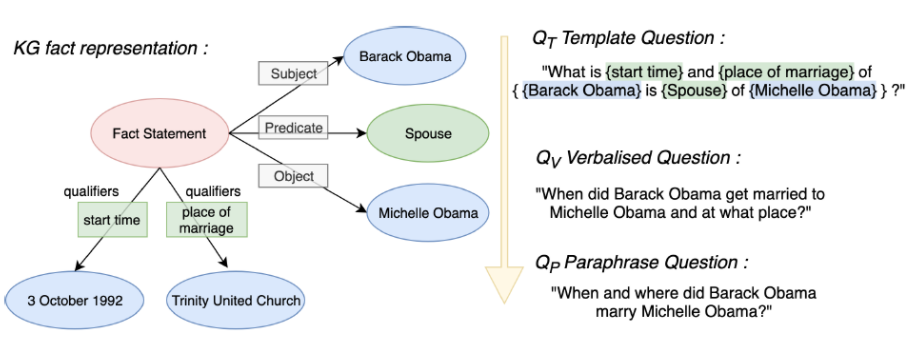
\includegraphics[scale=.55]{imagenes/2_theorical_framework/question_answering/lcquad2Workflow.PNG}
    \caption{Example of \LCQuADtwo{} question workflow generation~\cite{dataset:lcquad2-DubeyBA019}.}
    \label{fig:lcquad2Pipeline}
\end{figure}

Then, a set of relevant entities and a predicate list is selected based on each \SPARQL{} template, 
meaning that each question type includes different entities and properties (e.g. the property 
\texttt{birthPlace} might not be used for questions that require counting). For each case, a 
subgraph is built based on three factors: an entity, the \SPARQL{} template, and one or more 
suitable predicates. From each subgraph a \SPARQL{} query is generated. Next, each \SPARQL{} query is 
transformed to a normalized natural language question, called a Question Template (QT), which is 
then verbalised and paraphrased in a three-step pipeline based on human turkers from the Amazon 
Mechanical Turk tool (a crowdsourcing tool to perform simple tasks on a large scale). 

The first step is to convert each QT into Verbalised Question (QV), where most of the 
grammatical errors and semantic inconsistencies of the QT are fixed. The second step is to 
paraphrase each QV, where the resulting Paraphrased Question (QP) should preserve the overall 
semantic meaning while changing its syntactic content and structure. An example of the entire 
generation of one case is illustrated in Figure~\ref{fig:lcquad2Pipeline}. The last step is a 
human verification where a comparison is done between each QT with its corresponding QP in 
order to measure the quality of the final result in terms of semantic similarity.

After the entire generation process, a dataset is provided with around 52\% complex questions 
and significant variation in their  question structure. There is, however, a small percentage 
of error derived from using a crowdsourcing tool~\cite{dataset:lcquad2-DubeyBA019}, with questions 
losing part of their semantic intent or questions that are poorly verbalized/paraphrased, which 
should be taken into consideration when using this dataset to train NSP-based models. 
